\documentclass[11pt,a4paper]{article}
\usepackage[T1]{fontenc}
\usepackage[utf8]{inputenc}
\usepackage{lmodern}
\usepackage{textcomp}
\usepackage[left=1.8cm,right=1.8cm,top=2.3cm,bottom=2.2cm,headheight=14pt,headsep=8pt]{geometry}
\usepackage{multicol}
\usepackage{xcolor}
\usepackage{fancyhdr}
\usepackage{graphicx}
\usepackage{array}
\usepackage{amsmath,amssymb}
\usepackage{setspace}
\usepackage{longtable}
\graphicspath{{../}}
\definecolor{ygreen}{RGB}{46,139,87}
\renewcommand{\normalsize}{\fontsize{10.9}{13.4}\selectfont}
\renewcommand{\familydefault}{\rmdefault}
\setlength{\parindent}{0pt}
\setlength{\columnsep}{0.8cm}
\setlength{\columnseprule}{0.4pt}
\setlength{\multicolsep}{3pt plus 1pt minus 1pt}
\renewcommand{\textsubscript}[1]{\ensuremath{_{\text{\fontsize{8}{8}\selectfont #1}}}}
\renewcommand{\textsuperscript}[1]{\ensuremath{^{\text{\fontsize{8}{8}\selectfont #1}}}}
\newcommand{\qn}[1]{\textbf{\fontsize{11.5}{13}\selectfont #1}}
\newcommand{\qsep}{\par\vspace{1pt}\noindent\rule{0pt}{0.4pt}\par\vspace{5pt}}
\newcommand{\fwrule}{\par\vspace{5pt}\noindent\rule{\linewidth}{1.4pt}\par\vspace{7pt}}
\newsavebox{\fitb}
\newcommand{\fitbox}[1]{\sbox{\fitb}{#1}\ifdim\wd\fitb>\linewidth\resizebox{\linewidth}{!}{\usebox{\fitb}}\else\usebox{\fitb}\fi}
\newcommand{\diqqat}[1]{\par\smallskip\noindent\textbf{Diqqat!} #1\par\medskip}
\newcommand{\javob}{\par\smallskip\noindent\textbf{Javob:} \rule[-2pt]{7.5cm}{0.4pt}\par\smallskip\noindent\textbf{Diqqat!} Javobingizni javoblar varaqasiga ko`chirib yozing.\par\medskip}
\pagestyle{fancy}
\fancyhf{}
\renewcommand{\headrulewidth}{0.4pt}
\fancyhead[L]{\textit{Milliy sertifikat 2026. Kimyo}}
\fancyhead[R]{12-variant}
\fancyfoot[L]{\fontsize{8}{9}\selectfont \textcopyright{} Colba maktabi, 2026}
\fancyfoot[C]{\thepage}
\fancypagestyle{first}{\fancyhf{}\renewcommand{\headrulewidth}{0pt}\fancyfoot[L]{\fontsize{8}{9}\selectfont \textcopyright{} Colba maktabi, 2026}\fancyfoot[C]{\thepage}}
\begin{document}
\normalsize
\thispagestyle{first}
\noindent\fcolorbox{ygreen}{white}{\parbox{\dimexpr\linewidth-2\fboxsep-2\fboxrule\relax}{%
\textbf{\fontsize{13}{15}\selectfont Nazorat testi}\ \textit{\fontsize{10}{12}\selectfont $\cdot$ Aralash test $\cdot$ 12-variant}\hfill
\begin{tabular}[t]{@{}r@{}}\textit{Milliy sertifikat 2026. Kimyo}\\ \textbf{\textit{\fontsize{8}{9}\selectfont Vaqt:}} \textit{\fontsize{10}{12}\selectfont 180 daqiqa}\end{tabular}}}
\par\medskip
\noindent\textit{Davriy jadvaldan foydalanish mumkin.}
\par\medskip
\begin{multicols}{2}
\noindent\qn{1.} Qaysi juftliklarda reaksiya boradi? 1) Pb va ZnCl\textsubscript{2}; 2) Al va CuSO\textsubscript{4}; 3) Zn va CuSO\textsubscript{4}; 4) Ag va CuSO\textsubscript{4}

\noindent A)~\textsl{1, 2} \hfill B)~\textsl{4} \hfill C)~\textsl{1, 2, 4} \hfill D)~\textsl{2, 3}\par
\qsep
\noindent\qn{2.} Jadvalda bog`lar hosil qiluvchi atomlarning elektrmanfiyliklari berilgan:
\begin{center}
\renewcommand{\arraystretch}{1.15}
\fitbox{\begin{tabular}{|c|c|c|}\hline
\textbf{Bog`} & \textbf{EM (1-atom)} & \textbf{EM (2-atom)} \\ \hline
H--Cl & 2,1 & 3 \\ \hline
H--O & 2,1 & 3,5 \\ \hline
H--F & 2,1 & 4 \\ \hline
C--O & 2,5 & 3,5 \\ \hline
\end{tabular}}
\end{center}
Qaysi bog` eng qutbli (eng ko`p ionli xarakterga ega)?

\noindent A)~\textsl{H--Cl} \hfill B)~\textsl{H--O} \hfill C)~\textsl{C--O} \hfill D)~\textsl{H--F}\par
\qsep
\noindent\qn{3.} Rasmda neytral atom elektron qavatlarining orbital diagrammasi (kataklar -- orbitallar, o`qlar -- elektronlar) berilgan.
\begin{center}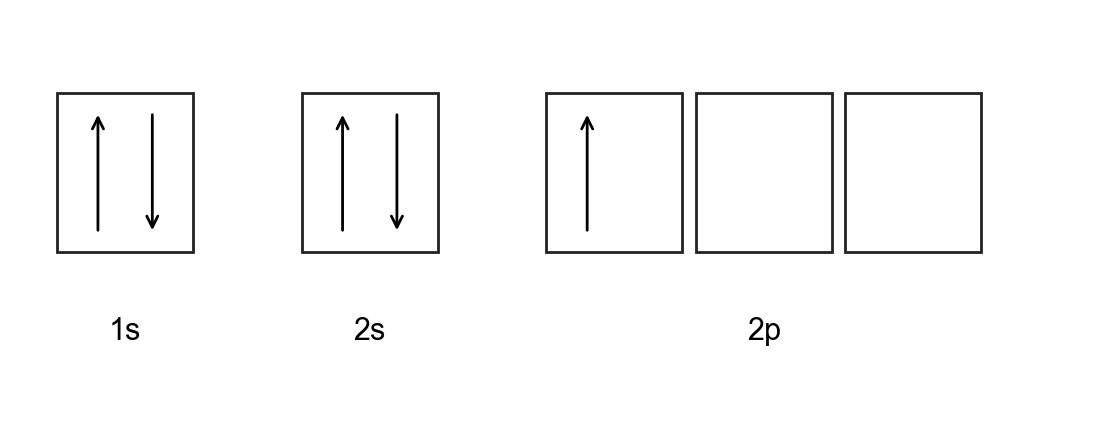
\includegraphics[width=0.86\linewidth]{rasmlar/gen/or_588848.png}\end{center}
Diagramma qaysi element atomiga tegishli?

\noindent A)~\textsl{kislorod} \hfill B)~\textsl{bor} \hfill C)~\textsl{azot} \hfill D)~\textsl{uglerod}\par
\qsep
\noindent\qn{4.} Gazlar aralashmasi tarkibi jadvalda berilgan (n.sh.):
\begin{center}
\renewcommand{\arraystretch}{1.15}
\fitbox{\begin{tabular}{|c|c|}\hline
\textbf{Gaz} & \textbf{Hajmi, l} \\ \hline
N\textsubscript{2} & 1 \\ \hline
H\textsubscript{2} & 1 \\ \hline
SO\textsubscript{2} & 3 \\ \hline
\end{tabular}}
\end{center}
Aralashmaning havoga nisbatan \textbf{zichligini aniqlang} (M(havo) = 29 g/mol).

\noindent A)~\textsl{3,06} \hfill B)~\textsl{0,77} \hfill C)~\textsl{1,53} \hfill D)~\textsl{44,4}\par
\qsep
\noindent\qn{5.} FeSO\textsubscript{4}$\cdot$7H\textsubscript{2}O kristallogidratida kristallizatsion suvning massa \textbf{ulushini (\%) aniqlang.}

\noindent A)~\textsl{54,7} \hfill B)~\textsl{22,7} \hfill C)~\textsl{82,9} \hfill D)~\textsl{45,3}\par
\qsep
\noindent\qn{6.} Konsentratsiyasi bir xil (0,1 mol/l) eritmalarning pH qiymatlari diagrammada berilgan.
\begin{center}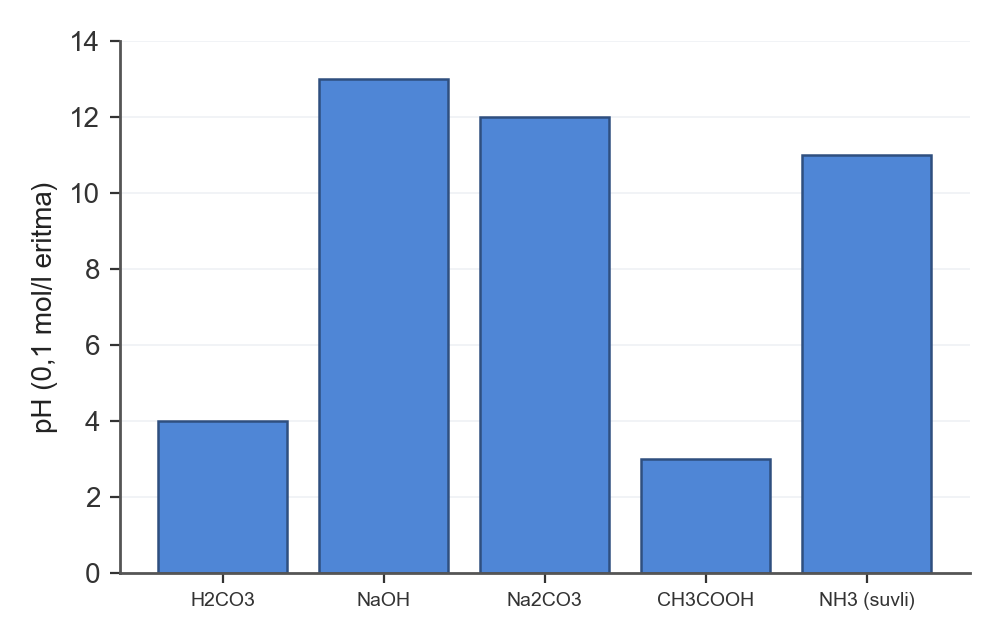
\includegraphics[width=0.86\linewidth]{rasmlar/gen/pb_v12_0.png}\end{center}
Qaysi eritmada [H\textsuperscript{+}] eng katta?

\noindent\begin{tabular}{@{}p{0.47\linewidth}@{}p{0.47\linewidth}@{}}
A)~\textsl{CH\textsubscript{3}COOH} & B)~\textsl{NH\textsubscript{3} (suvli)} \\
C)~\textsl{Na\textsubscript{2}CO\textsubscript{3}} & D)~\textsl{H\textsubscript{2}CO\textsubscript{3}} \\
\end{tabular}\par
\qsep
\noindent\qn{7.} Fosfor (\textit{Z} = 15) atomida nechta juftlashmagan elektron bor?

\noindent A)~\textsl{4} \hfill B)~\textsl{2} \hfill C)~\textsl{5} \hfill D)~\textsl{3}\par
\qsep
\noindent\qn{8.} 4 g NaOH ni to`liq neytrallash uchun 6 g CH\textsubscript{3}COOH sarflandi. CH\textsubscript{3}COOH ning ekvivalent \textbf{massasini (g/mol) aniqlang.}

\noindent A)~\textsl{60} \hfill B)~\textsl{120} \hfill C)~\textsl{30} \hfill D)~\textsl{6}\par
\qsep
\noindent\qn{9.} 100 g 10\% li MgSO\textsubscript{4} eritmasiga 50 g shu tuzning o`zi qo`shilib eritildi. Hosil bo`lgan eritmaning massa \textbf{ulushini (\%) aniqlang.}

\noindent A)~\textsl{40} \hfill B)~\textsl{60} \hfill C)~\textsl{30} \hfill D)~\textsl{32}\par
\qsep
\noindent\qn{10.} 1,5 mol H\textsubscript{2}O tarkibida necha mol atom bor?

\noindent A)~\textsl{3} \hfill B)~\textsl{4,5} \hfill C)~\textsl{6} \hfill D)~\textsl{1,5}\par
\qsep
\noindent\qn{11.} Fe plastinka 8 g CuSO\textsubscript{4} ni tutgan eritmaga tushirildi va Cu to`liq ajralib chiqquncha ushlab turildi. Plastinka massasi necha gramm ortadi?

\noindent A)~\textsl{0,4} \hfill B)~\textsl{0,8} \hfill C)~\textsl{0,2} \hfill D)~\textsl{8}\par
\qsep
\noindent\qn{12.} H\textsubscript{3}PO\textsubscript{3} tarkibida P ning oksidlanish \textbf{darajasini aniqlang.}

\noindent A)~\textsl{+3} \hfill B)~\textsl{$-$1} \hfill C)~\textsl{+3 va +5} \hfill D)~\textsl{+4}\par
\qsep
\noindent\qn{13.} Mishyak (\textit{Z} = 33) atomi elektron konfiguratsiyasida jami nechta juftlashgan elektron bor?

\noindent A)~\textsl{31} \hfill B)~\textsl{29} \hfill C)~\textsl{30} \hfill D)~\textsl{32}\par
\qsep
\noindent\qn{14.} Qaysi juftliklar o`zaro reaksiyaga kirishadi? 1) Fe va HCl; 2) Fe\textsubscript{2}O\textsubscript{3} va H\textsubscript{2}O; 3) CuSO\textsubscript{4} va NaOH; 4) CuO va H\textsubscript{2}

\noindent A)~\textsl{1, 2, 4} \hfill B)~\textsl{2, 3} \hfill C)~\textsl{1, 3, 4} \hfill D)~\textsl{1, 3}\par
\qsep
\noindent\qn{15.} Cu(NO\textsubscript{3})\textsubscript{2} qizdirilganda qanday moddalar hosil bo`ladi?

\noindent\begin{tabular}{@{}p{0.47\linewidth}@{}p{0.47\linewidth}@{}}
A)~\textsl{CuO, NO\textsubscript{2} va O\textsubscript{2}} & B)~\textsl{ZnO, NO\textsubscript{2} va O\textsubscript{2}} \\
C)~\textsl{Ag, NO\textsubscript{2} va O\textsubscript{2}} & D)~\textsl{NaNO\textsubscript{2} va O\textsubscript{2}} \\
\end{tabular}\par
\qsep
\noindent\qn{16.} 6,2 g fosfor yondirilib, hosil bo`lgan oksid suvda eritildi (ortofosfat kislota), so`ng 0,3 mol NaOH qo`shildi. Hosil bo`lgan NaH\textsubscript{2}PO\textsubscript{4} \textbf{massasini (g) aniqlang.}

\noindent A)~\textsl{24} \hfill B)~\textsl{6} \hfill C)~\textsl{12} \hfill D)~\textsl{32,8}\par
\qsep
\noindent\qn{17.} 2NaBr + Cl\textsubscript{2} $\to$ 2NaCl + Br\textsubscript{2} jarayoni uchun 22,4 l (n.sh.) Cl\textsubscript{2} olingan (unum 75\%). Br\textsubscript{2} \textbf{massasini (g) aniqlang.}

\noindent A)~\textsl{160} \hfill B)~\textsl{120} \hfill C)~\textsl{240} \hfill D)~\textsl{60}\par
\qsep
\noindent\qn{18.} Li va Na dan iborat 6,7 g aralashma suv bilan reaksiyaga kirishdi. Ajralgan vodorodning \textbf{hajmini (l, n.sh.) aniqlang.}

\noindent A)~\textsl{11,2} \hfill B)~\textsl{2,8} \hfill C)~\textsl{5,6} \hfill D)~\textsl{3,35}\par
\qsep
\noindent\qn{19.} Alyuminiy va rux dan iborat 18,4 g aralashma mo`l xlorid kislotada eritilganda 11,2 l (n.sh.) vodorod ajraldi. Aralashmadagi alyuminiyning massa \textbf{ulushini (\%) aniqlang.}

\noindent A)~\textsl{70,7} \hfill B)~\textsl{29,3} \hfill C)~\textsl{14,7} \hfill D)~\textsl{5,4}\par
\qsep
\noindent\qn{20.} Uglevodorodning 4,4 g massasi yondirilganda 13,2 g CO\textsubscript{2} va 7,2 g H\textsubscript{2}O hosil bo`ldi. Uglevodorod molekulasidagi uglerod atomlari \textbf{sonini toping} (M = 44 g/mol).

\noindent A)~\textsl{4} \hfill B)~\textsl{3} \hfill C)~\textsl{2} \hfill D)~\textsl{8}\par
\qsep
\noindent\qn{21.} CH\textsubscript{3}--CH\textsubscript{2}--CH(CH\textsubscript{3})--CHO birikmaning sistematik nomi qaysi qatorda to`g`ri keltirilgan?

\noindent\begin{tabular}{@{}p{0.47\linewidth}@{}p{0.47\linewidth}@{}}
A)~\textsl{3-metilbutanal} & B)~\textsl{2-metilbutanal} \\
C)~\textsl{pentanal} & D)~\textsl{2-metilbutanon} \\
\end{tabular}\par
\qsep
\noindent\qn{22.} 6,5 g C\textsubscript{2}H\textsubscript{2} dan quyidagi ikki bosqichda C\textsubscript{2}H\textsubscript{5}OH olinadi: 1) C\textsubscript{2}H\textsubscript{2} + H\textsubscript{2}O $\to$ CH\textsubscript{3}CHO (unum 80\%); 2) CH\textsubscript{3}CHO + H\textsubscript{2} $\to$ C\textsubscript{2}H\textsubscript{5}OH (unum 50\%). Oxirgi mahsulot C\textsubscript{2}H\textsubscript{5}OH ning \textbf{massasini (g) toping.}

\noindent A)~\textsl{5,75} \hfill B)~\textsl{9,2} \hfill C)~\textsl{11,5} \hfill D)~\textsl{4,6}\par
\qsep
\noindent\qn{23.} CH\textsubscript{3}COONa + NaOH (t) reaksiyasi natijasida qaysi organik modda hosil bo`ladi?

\noindent\begin{tabular}{@{}p{0.47\linewidth}@{}p{0.47\linewidth}@{}}
A)~\textsl{sirka aldegid} & B)~\textsl{metan} \\
C)~\textsl{etilen} & D)~\textsl{benzoy kislota} \\
\end{tabular}\par
\qsep
\noindent\qn{24.} Aldegid va ketonlar haqida qaysi fikrlar to`g`ri? 1) Aseton Cu(OH)\textsubscript{2} ni qaytaradi; 2) Aldegidlar "kumush ko`zgu" reaksiyasini beradi; 3) Ketonlar kuchsiz oksidlovchilar bilan oksidlanmaydi; 4) Formalin --- formaldegidning 40\% li eritmasi

\noindent A)~\textsl{1, 2, 3} \hfill B)~\textsl{2, 3, 4} \hfill C)~\textsl{1, 3, 4} \hfill D)~\textsl{2, 4}\par
\qsep
\noindent\qn{25.} Reaksiya tenglamasi: C\textsubscript{2}H\textsubscript{5}COOH + KOH $\to$ C\textsubscript{2}H\textsubscript{5}COOK + H\textsubscript{2}O. Reaksiyaga 56 g KOH kirishdi. C\textsubscript{2}H\textsubscript{5}COOH \textbf{miqdorini (mol) hisoblang.}

\noindent A)~\textsl{2} \hfill B)~\textsl{0,5} \hfill C)~\textsl{1,5} \hfill D)~\textsl{1}\par
\qsep
\noindent\qn{26.} Murakkab efirlar va yog`lar haqida qaysi fikrlar to`g`ri? 1) Suyuq yog`lar to`yinmagan kislotalardan hosil bo`lgan; 2) Etilatsetat efir hidli suyuqlik; 3) Murakkab efirlarning gidrolizi ishqoriy muhitda qaytmas; 4) Dietil efir spirtdan yuqori haroratda qaynaydi

\noindent A)~\textsl{2, 3, 4} \hfill B)~\textsl{1, 4} \hfill C)~\textsl{1, 2, 3} \hfill D)~\textsl{1, 3, 4}\par
\qsep
\noindent\qn{27.} Quyidagi birikmalardan qaysi biri aldegid sinfiga kiradi?

\noindent\begin{tabular}{@{}p{0.47\linewidth}@{}p{0.47\linewidth}@{}}
A)~\textsl{CH\textsubscript{3}CHO} & B)~\textsl{CH\textsubscript{3}COCH\textsubscript{3}} \\
C)~\textsl{C\textsubscript{6}H\textsubscript{5}OH} & D)~\textsl{H\textsubscript{2}NCH\textsubscript{2}COOH} \\
\end{tabular}\par
\qsep
\noindent\qn{28.} Quyidagi birikmalardan qaysi biri murakkab efir sinfiga kiradi?

\noindent\begin{tabular}{@{}p{0.47\linewidth}@{}p{0.47\linewidth}@{}}
A)~\textsl{C\textsubscript{6}H\textsubscript{5}OH} & B)~\textsl{CH\textsubscript{3}COOH} \\
C)~\textsl{CH\textsubscript{3}COOC\textsubscript{2}H\textsubscript{5}} & D)~\textsl{CH\textsubscript{3}CHO} \\
\end{tabular}\par
\qsep
\noindent\qn{29.} Yuqori molekulyar birikmalar haqida qaysi fikrlar to`g`ri? 1) Kapron poliamid tola; 2) Teflon --- polivinilxlorid; 3) Fenolformaldegid smola polikondensatsiya mahsuloti; 4) Polimerning M = zveno M $\cdot$ polimerlanish darajasi

\noindent A)~\textsl{1, 3} \hfill B)~\textsl{3, 4} \hfill C)~\textsl{2, 3, 4} \hfill D)~\textsl{1, 3, 4}\par
\qsep
\noindent\qn{30.} Uch probirkada (\textit{X}, \textit{Y}, \textit{Z}) NaCl, NaBr, NaI eritmalari bor (tartibsiz). Ularga AgNO\textsubscript{3} ta'sir ettirildi. Kuzatuvlar jadvalda:
\begin{center}
\renewcommand{\arraystretch}{1.15}
\fitbox{\begin{tabular}{|c|c|}\hline
\textbf{Probirka} & \textbf{AgNO\textsubscript{3} qo`shilganda} \\ \hline
\textit{X} & och sariq cho`kma \\ \hline
\textit{Y} & oq cho`kma \\ \hline
\textit{Z} & sariq cho`kma \\ \hline
\end{tabular}}
\end{center}
\textit{X}, \textit{Y}, \textit{Z} probirkalardagi \textbf{moddalarni aniqlang.}
\noindent A)~\textsl{\textit{X} -- NaBr, \textit{Y} -- NaCl, \textit{Z} -- NaI}\par
\noindent B)~\textsl{\textit{X} -- NaI, \textit{Y} -- NaCl, \textit{Z} -- NaBr}\par
\noindent C)~\textsl{\textit{X} -- NaBr, \textit{Y} -- NaI, \textit{Z} -- NaCl}\par
\noindent D)~\textsl{\textit{X} -- NaCl, \textit{Y} -- NaBr, \textit{Z} -- NaI}\par
\qsep
\noindent\qn{31.} Kimyo laboratoriyasida ishlash qoidalari haqida qaysi fikrlar to`g`ri? 1) Kuygan joy ko`p suv bilan yuviladi; 2) Ishqor teriga tushsa, qo`l suv bilan yuviladi; 3) Zaharli gaz ajraladigan tajriba mo`rili shkafda o`tkaziladi; 4) Konsentrlangan kislotani suvga ohista, aralashtirib quyiladi

\noindent\begin{tabular}{@{}p{0.47\linewidth}@{}p{0.47\linewidth}@{}}
A)~\textsl{1, 2, 3} & B)~\textsl{1, 3, 4} \\
C)~\textsl{2, 3, 4} & D)~\textsl{1, 2, 3, 4} \\
\end{tabular}\par
\qsep
\noindent\qn{32.} Rasmda aralashmani ajratish usuli ko`rsatilgan. Bu \textbf{usulni toping.}
\begin{center}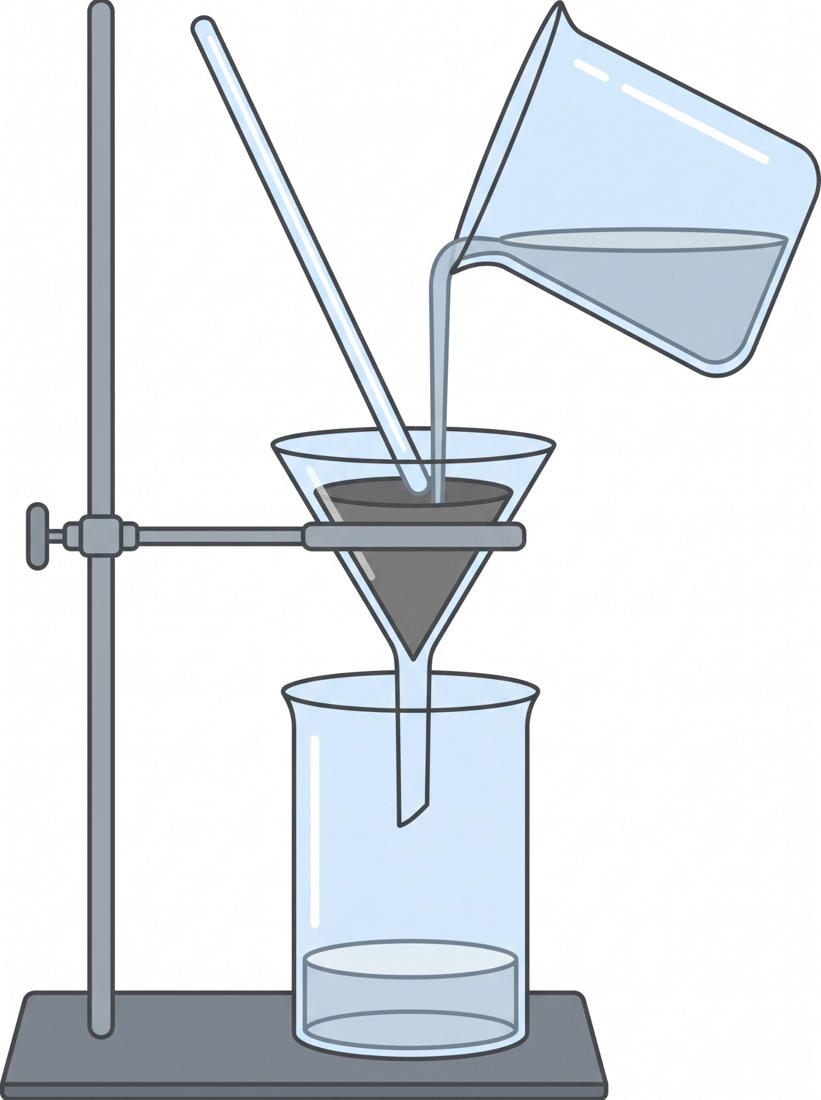
\includegraphics[width=0.86\linewidth]{rasmlar/darslik/d_filtr.png}\end{center}
\noindent A)~\textsl{distillash}\par
\noindent B)~\textsl{magnit yordamida ajratish}\par
\noindent C)~\textsl{filtrlash}\par
\noindent D)~\textsl{bug`latish   ---}\par
\qsep
\end{multicols}
\medskip
\noindent\setlength{\fboxsep}{0pt}\fbox{\begin{tabular}{p{0.74\linewidth}|p{0.2\linewidth}}
\parbox[t]{0.72\linewidth}{\vspace{3pt}\textbf{Topshiriqlar (33--35) va javob variant (A--F)larini o`zaro to`g`ri moslashtiring.} Alyuminiy va temir (Al va Fe) dan iborat 12,45 g qotishma mo`l H\textsubscript{2}SO\textsubscript{4} eritmasida eritilganda 8,4 l (n.sh.) gaz ajraldi.
\vspace{3pt}} & \parbox[t]{0.19\linewidth}{\vspace{3pt}A~\textsl{48,45}\\[3pt]
B~\textsl{183,75}\\[3pt]
C~\textsl{48,8}\\[3pt]
D~\textsl{91,88}\\[3pt]
E~\textsl{32,53}\\[3pt]
F~\textsl{38,76}}\\ \hline
\parbox[t]{0.72\linewidth}{\vspace{2pt}\textbf{33. Qotishmadagi Al massa ulushini (\%) aniqlang.}\vspace{2pt}} & \\ \hline
\parbox[t]{0.72\linewidth}{\vspace{2pt}\textbf{34. Reaksiya uchun sarflangan 20\% li H\textsubscript{2}SO\textsubscript{4} massasini (g) aniqlang.}\vspace{2pt}} & \\ \hline
\parbox[t]{0.72\linewidth}{\vspace{2pt}\textbf{35. Eritmadagi tuzlarning umumiy massasini (g) aniqlang.}\vspace{2pt}} & 
\end{tabular}}
\par\bigskip
\noindent\qn{36.} Fe + H\textsubscript{2}SO\textsubscript{4} $\to$ Fe\textsubscript{2}(SO\textsubscript{4})\textsubscript{3} + SO\textsubscript{2} + H\textsubscript{2}O reaksiya tenglamasini tenglang. Oksidlovchi va qaytaruvchi oldidagi koeffitsiyentlar \textbf{yig`indisini aniqlang.}
\javob\qsep
\noindent\qn{37.} CuSO\textsubscript{4} eritmasi inert elektrodlar yordamida 2 A tok kuchi bilan 9650 s elektroliz qilindi. Katodda ajralgan Cu massasi (g) \textbf{ni toping.}
\javob\qsep
\noindent\qn{38.} CaCO\textsubscript{3} va MgCO\textsubscript{3} dan iborat 18,4 g aralashma doimiy massagacha qizdirilganda qoldiq massasi 9,6 g bo`ldi. Aralashmadagi CaCO\textsubscript{3} ning \textbf{massasini (g) toping.}
\javob\qsep
\noindent\qn{39.} 4,4 g etanal Ag\textsubscript{2}O ning ammiakli eritmasi bilan to`liq oksidlanganda hosil bo`lgan kumush \textbf{massasini (g) aniqlang.}
\javob\qsep
\noindent\qn{40.} 1,5 mol asetilendan Zelinskiy usuli bilan (100\% unum) benzol olindi. Benzol \textbf{massasini (g) aniqlang.}
\javob\qsep
\par\bigskip\begin{center}\textbf{\fontsize{13}{15}\selectfont YOZMA ISH}\end{center}
\noindent\qn{41.} \textbf{Topshiriqni bajarish jarayonida barcha reaksiya tenglamalarini yozing. Miqdoriy va arifmetik hisoblashlarni (unga asos bo`lgan usul yoki formulani ko`rsatgan holda) uzviy ketma-ketlikda bajaring.}\par\smallskip
14,35 g ZnSO\textsubscript{4}$\cdot$7H\textsubscript{2}O 400 g suvda eritildi.\par
\noindent 1)Hosil bo`lgan eritmadagi ZnSO\textsubscript{4} ning massa ulushini (\%) toping.\par
\noindent 2)Eritmaga mo`l BaCl\textsubscript{2} eritmasi qo`shildi. Hosil bo`lgan cho`kma massasini (g) toping. Eritmadagi kation miqdorini (mol) ham toping.\par
\noindent 3)Xuddi shunday eritmaga ekvivalent miqdorda NaOH qo`shilganda hosil bo`lgan Zn(OH)\textsubscript{2} cho`kmasining massasini (g) toping.\par
\noindent 4)Eritmaga Mg plastinka tushirildi (ZnSO\textsubscript{4} tuzidagi metall to`liq siqib chiqarildi). Plastinka massasi qanchaga (g) o`zgargan? Dastlabki eritma massasini (g) ham ayting.\par
\noindent 5)Kristallogidratdagi kristallizatsion suvning massa ulushini (\%) va unda suv molekulalari sonini toping. Shu miqdor kristallogidrat suvsizlantirilganda massa necha gramm kamayadi?\par
\diqqat{Mazkur topshiriq kengaytirilgan javobni talab etib, uning yechilish usuli va shu usul asosidagi barcha hisoblash amallari javoblar varaqasida aks etishi lozim.}\qsep
\noindent\qn{42.} Reaksiya tenglamalarini tugallang va tenglang. Hosil bo`lgan organik moddalarning tuzilish formulalarini yozing va ularni nomlang.\par
\noindent 1)CH\textsubscript{3}COOCH\textsubscript{3} + NaOH $\xrightarrow{\text{t}}$\par
\noindent 2)CH\textsubscript{3}COOH + NaHCO\textsubscript{3} $\to$\par
\noindent 3)CH\textsubscript{4} + Cl\textsubscript{2} $\xrightarrow{\text{yorug`lik}}$\par
\noindent 4)CH\textsubscript{2}=CH\textsubscript{2} + Br\textsubscript{2} $\to$\par
\noindent 5)C\textsubscript{6}H\textsubscript{5}NO\textsubscript{2} + H\textsubscript{2} $\xrightarrow{\text{kat.}}$\par
\noindent 6)C\textsubscript{2}H\textsubscript{5}OH $\xrightarrow{\text{H\textsubscript{2}SO\textsubscript{4}(kons.), 170 \textdegree{}C}}$\par
\noindent 7)CH\textsubscript{3}CHO + Ag\textsubscript{2}O $\xrightarrow{\text{NH\textsubscript{3}, t}}$\par
\diqqat{Mazkur topshiriq kengaytirilgan javobni talab etib, uning yechilish usuli va shu usul asosidagi barcha hisoblash amallari javoblar varaqasida aks etishi lozim.}\qsep
\noindent\qn{43.} \textbf{Topshiriqni bajarish jarayonida barcha reaksiya tenglamalarini yozing. Miqdoriy va arifmetik hisoblashlarni (unga asos bo`lgan usul yoki formulani ko`rsatgan holda) uzviy ketma-ketlikda bajaring.}\par\smallskip
75,2 g Cu(NO\textsubscript{3})\textsubscript{2} qizdirilganda qisman parchalandi va qattiq qoldiq massasi 64,4 g bo`ldi. Ajralgan gazlar aralashmasi 300 g suvga to`liq yuttirildi. Qattiq qoldiq esa CuO ni to`liq eritadigan (ortiqcha bo`lmagan) miqdordagi suyultirilgan H\textsubscript{2}SO\textsubscript{4} da eritildi, hosil bo`lgan eritmaga temir qipig`i solindi.\par
\noindent 1)Parchalanish reaksiyasi tenglamasini yozing. Parchalangan Cu(NO\textsubscript{3})\textsubscript{2} ning ulushini (\%) va ajralgan gazlar hajmini (l, n.sh.) aniqlang.\par
\noindent 2)Qattiq qoldiqdagi CuO ning massa ulushini (\%) hisoblang.\par
\noindent 3)Gazlar suvga yuttirilganda hosil bo`lgan eritmadagi HNO\textsubscript{3} ning massa ulushini (\%) toping (reaksiya tenglamasini yozing).\par
\noindent 4)Temir qipig`i eritmadagi barcha Cu\textsuperscript{2+} ionlarini siqib chiqarishi uchun zarur temir massasini (g) va ajralgan mis massasini (g) aniqlang (reaksiya tenglamalarini yozing).\par
\noindent 5)Ajralgan NO\textsubscript{2} va O\textsubscript{2} gazlari aralashmasining o`rtacha molyar massasini (g/mol) hisoblang.\par
\diqqat{Mazkur topshiriq kengaytirilgan javobni talab etib, uning yechilish usuli va shu usul asosidagi barcha hisoblash amallari javoblar varaqasida aks etishi lozim.}\qsep
\newpage
\noindent\textbf{\fontsize{13}{15}\selectfont Nazorat testi}\ \textit{$\cdot$ 12-variant}\hfill \textbf{Javoblar kaliti}\par\smallskip\hrule\smallskip
\textit{Faqat o`qituvchi uchun.}\par\medskip
\noindent\textbf{1--32-savollar}\par\smallskip
\noindent\begin{tabular}{|c|c|c|c|c|c|c|c|c|c|c|c|c|c|c|c|}\hline
\textbf{1} & \textbf{2} & \textbf{3} & \textbf{4} & \textbf{5} & \textbf{6} & \textbf{7} & \textbf{8} & \textbf{9} & \textbf{10} & \textbf{11} & \textbf{12} & \textbf{13} & \textbf{14} & \textbf{15} & \textbf{16}\\\hline
\textsl{D} & \textsl{D} & \textsl{B} & \textsl{C} & \textsl{D} & \textsl{A} & \textsl{D} & \textsl{A} & \textsl{A} & \textsl{B} & \textsl{A} & \textsl{A} & \textsl{C} & \textsl{C} & \textsl{A} & \textsl{C}\\\hline
\textbf{17} & \textbf{18} & \textbf{19} & \textbf{20} & \textbf{21} & \textbf{22} & \textbf{23} & \textbf{24} & \textbf{25} & \textbf{26} & \textbf{27} & \textbf{28} & \textbf{29} & \textbf{30} & \textbf{31} & \textbf{32}\\\hline
\textsl{B} & \textsl{C} & \textsl{B} & \textsl{B} & \textsl{B} & \textsl{D} & \textsl{B} & \textsl{B} & \textsl{D} & \textsl{C} & \textsl{A} & \textsl{C} & \textsl{D} & \textsl{A} & \textsl{D} & \textsl{C}\\\hline
\end{tabular}\par\medskip
\noindent\textbf{33--35-savollar}\par\smallskip
\noindent\begin{tabular}{|c|c|c|}\hline \textbf{No} & \textbf{Javob} & \textbf{Qiymat}\\\hline
33 & \textsl{E} & 32,53\\\hline
34 & \textsl{B} & 183,75\\\hline
35 & \textsl{A} & 48,45\\\hline
\end{tabular}\par\medskip
\noindent\textbf{36--40-savollar}\par\smallskip
\noindent\begin{tabular}{|c|c|}\hline \textbf{No} & \textbf{To`g`ri javob}\\\hline
36 & 8\\\hline
37 & 6,4\\\hline
38 & 10\\\hline
39 & 21,6\\\hline
40 & 39\\\hline
\end{tabular}\par\medskip
\noindent\textbf{41--43-topshiriqlar: javoblar}\par\smallskip
\noindent\textbf{41-topshiriq.}\par
\noindent 1) 1,94\%\par
\noindent 2) 11,65 g; 0,05 mol\par
\noindent 3) 4,95 g\par
\noindent 4) 2,05 g; 414,35 g\par
\noindent 5) 43,9\%; 7; 6,3 g\par
\noindent\textbf{42-topshiriq.}\par
\noindent 1) CH\textsubscript{3}COOCH\textsubscript{3} + NaOH $\xrightarrow{\text{t}}$ CH\textsubscript{3}COONa + CH\textsubscript{3}OH --- natriy atsetat va metanol (4 ball)\par
\noindent 2) CH\textsubscript{3}COOH + NaHCO\textsubscript{3} $\to$ CH\textsubscript{3}COONa + H\textsubscript{2}O + CO\textsubscript{2} --- natriy atsetat (4 ball)\par
\noindent 3) CH\textsubscript{4} + Cl\textsubscript{2} $\xrightarrow{\text{yorug`lik}}$ CH\textsubscript{3}Cl + HCl --- xlormetan (3 ball)\par
\noindent 4) CH\textsubscript{2}=CH\textsubscript{2} + Br\textsubscript{2} $\to$ CH\textsubscript{2}Br--CH\textsubscript{2}Br --- 1,2-dibrometan (4 ball)\par
\noindent 5) C\textsubscript{6}H\textsubscript{5}NO\textsubscript{2} + H\textsubscript{2} $\xrightarrow{\text{kat.}}$ C\textsubscript{6}H\textsubscript{5}NH\textsubscript{2} + H\textsubscript{2}O --- anilin (3 ball)\par
\noindent 6) C\textsubscript{2}H\textsubscript{5}OH $\xrightarrow{\text{H\textsubscript{2}SO\textsubscript{4}(kons.), 170 \textdegree{}C}}$ CH\textsubscript{2}=CH\textsubscript{2} + H\textsubscript{2}O --- etilen (3 ball)\par
\noindent 7) CH\textsubscript{3}CHO + Ag\textsubscript{2}O $\xrightarrow{\text{NH\textsubscript{3}, t}}$ CH\textsubscript{3}COOH + 2Ag$\downarrow$ --- etan (sirka) kislota (4 ball)\par
\noindent\textbf{43-topshiriq.}\par
\noindent 1) 25\%; 5,6 l\par
\noindent 2) 12,4\%\par
\noindent 3) 4,05\%\par
\noindent 4) 22,4 g; 25,6 g\par
\noindent 5) 43,2 g/mol\par
\par\bigskip\noindent\textbf{Mavzular taqsimoti}\par\smallskip
{\small\noindent\begin{longtable}{|c|p{7.2cm}|p{5.4cm}|c|}\hline \textbf{No} & \textbf{Mavzu} & \textbf{Tekshiriladigan ko`nikma} & \textbf{Ball}\\\hline
1 & Tashev; 9-sinf (kuchlanish qatori) & Bilim va tushunish & 1\\\hline
2 & 8-sinf (kimyoviy bog`lanish turlari, jadval) & Jadval tahlili & 1\\\hline
3 & 8-sinf (elektron konfiguratsiya, orbital diagramma) & Rasm bo`yicha tahlil & 1\\\hline
4 & 11-sinf (gaz aralashmalar, jadval) & Jadval tahlili & 1\\\hline
5 & 7-sinf; Tirkashev (kristallogidrat) & Hisoblash va masala yechish & 1\\\hline
6 & Tirkashev \textit{V} bob (pH, diagramma) & Grafik tahlili & 1\\\hline
7 & Tirkashev I bob; 8-sinf (elektron konfiguratsiya) & Bilim va tushunish & 1\\\hline
8 & 11-sinf (ekvivalentlar qonuni) & Hisoblash va masala yechish & 1\\\hline
9 & Tirkashev III bob (eritmalar) & Hisoblash va masala yechish & 1\\\hline
10 & 7-sinf (mol) & Hisoblash va masala yechish & 1\\\hline
11 & Tashev; 9-sinf (metallarning kuchlanish qatori) & Hisoblash va masala yechish & 1\\\hline
12 & 8-sinf; Tirkashev \textit{V} bob (oksidlanish darajasi) & Bilim va tushunish & 1\\\hline
13 & Tirkashev I bob (kvant sonlari) & Bilim va tushunish & 1\\\hline
14 & 9-sinf; Tashev (anorganik birikmalar xossalari) & Bilim va tushunish & 1\\\hline
15 & Tashev (nitratlar) & Bilim va tushunish & 1\\\hline
16 & Tashev (fosfor) & Hisoblash va masala yechish & 1\\\hline
17 & 9-sinf; Tirkashev (galogenlar, hisob) & Hisoblash va masala yechish & 1\\\hline
18 & 9-sinf (ishqoriy metallar) & Hisoblash va masala yechish & 1\\\hline
19 & 9-sinf (Al, Mg, Ca) & Hisoblash va masala yechish & 1\\\hline
20 & 10-sinf (formulani aniqlash) & Hisoblash va masala yechish & 1\\\hline
21 & 10-sinf (nomenklatura \S{}6, \S{}11, \S{}20, \S{}24--26) & Bilim va tushunish & 1\\\hline
22 & 10-sinf (ikki bosqichli hisob) & Hisoblash va masala yechish & 1\\\hline
23 & 10-sinf (olinish usullari) & Bilim va tushunish & 1\\\hline
24 & 10-sinf (mavzuga oid paragraflar); Abdusamatov & Bilim va tushunish & 1\\\hline
25 & 10-sinf (kis, hisob) & Hisoblash va masala yechish & 1\\\hline
26 & 10-sinf (mavzuga oid paragraflar); Abdusamatov & Bilim va tushunish & 1\\\hline
27 & 10-sinf (organik birikmalar sinflari) & Bilim va tushunish & 1\\\hline
28 & 10-sinf (organik birikmalar sinflari) & Bilim va tushunish & 1\\\hline
29 & 10-sinf (mavzuga oid paragraflar); Abdusamatov & Bilim va tushunish & 1\\\hline
30 & 7--10-sinf va Tashev (laboratoriya ishlari, sifat reaksiyalar) & Jadval tahlili & 1\\\hline
31 & 7-sinf (xavfsizlik qoidalari); 10-sinf lab. & Bilim va tushunish & 1\\\hline
32 & 7-sinf (11-rasm) & Rasm bo`yicha tahlil & 1\\\hline
33--35 & Aralash masala (moslashtirish) & Ko`p bosqichli hisob & 3\\\hline
36--40 & Qisqa javobli masalalar & Hisoblash & 5\\\hline
41--43 & Yozma ish & Usul va hisob (M, A) & 75\\\hline
\end{longtable}}
\end{document}
